%\documentclass{article}
\documentclass[12pt]{article}

% --------------------------------
% MARGINS

%\textwidth 6.5in
%\textheight 9.0in
%\voffset=-0.40in
%\voffset=-0.8in % to account for northern slide in pdf
% \hoffset=-.90in
%\hoffset=-0.84in % to account for eastern slide in pdf

% --------------------------------
% PACKAGES

\usepackage{multicol}
\usepackage{amsmath,amsfonts,amsthm,amssymb}
\usepackage{graphicx}
\usepackage{tikz}
\usepackage{enumitem}
\usepackage{verbatim}
\usepackage{color}
\usepackage{xcolor}
\usepackage[normalem]{ulem}
\usepackage{comment,nicefrac}
\usepackage{setspace}

% --------------------------------
% THEOREMS

\newtheorem{thm}{Theorem}
\newtheorem{clm}[thm]{Claim}
\newtheorem{cnj}[thm]{Conjecture}
\newtheorem{cor}[thm]{Corollary}
\newtheorem{fct}[thm]{Fact}
\newtheorem{lem}[thm]{Lemma}
\newtheorem{qst}[thm]{Question}
\newtheorem{prop}[thm]{Proposition}

% --------------------------------
% COLORS

\definecolor{brwn}{RGB}{140, 70, 20}
\definecolor{gren}{RGB}{  0,140, 10}

% --------------------------------
% NUMBERS

\pgfmathsetmacro\Radi{6}
\pgfmathsetmacro\radi{3}

% --------------------------------
% LETTERS

\def\bT{{\boldsymbol{T}}}


% **************************************************
% DOCUMENT
% **************************************************
\begin{document}

\title{On the pebbling numbers of some snarks} 

\author{
Matheus Adauto \footnotemark[1]\ \footnotemark[4]
\and
Mariana da Cruz \footnotemark[1]\ \footnotemark[5]
\and
Celina de Figueiredo \footnotemark[1]\ \footnotemark[6]
\and
Glenn Hurlbert \footnotemark[2]
\and
Diana Sasaki \footnotemark[3]
}
\date{}
\maketitle

\footnotetext[1]{
Programa de Engenharia de Sistemas e Computa\c{c}{\~a}o, 
Universidade Federal do Rio de Janeiro, 
Rio de Janeiro, Brazil
}

\footnotetext[2]{
Department of Mathematics and Applied Mathematics,
Virginia Commonwealth University, 
Richmond, VA, USA,
\texttt{ghurlbert@vcu.edu}
}

\footnotetext[3]{
Instituto de Matem{\'a}tica e Estat{\'i}stica, 
Universidade do Estado do Rio de Janeiro, 
Brazil,
\texttt{diana.sasaki@ime.uerj.br}
}

\footnotetext[4]{
\texttt{adauto@cos.ufrj.br}
}

\footnotetext[5]{
\texttt{mmartins@cos.ufrj.br}
}

\footnotetext[6]{
\texttt{celina@cos.ufrj.br}
}

\date{}

\maketitle


%%%%%%%%%%%%%%%%%%%%%%%%%%%%%%%%%%%%%%%%%%%%%%%
%       ABSTRACT
%%%%%%%%%%%%%%%%%%%%%%%%%%%%%%%%%%%%%%%%%%%%%%%
\begin{abstract}
Graph pebbling is a game played on graphs with pebbles on their vertices. 
A pebbling move removes two pebbles from one vertex and places one pebble on an adjacent vertex. 
The pebbling number $\pi(G)$ is the smallest $t$ so that from any initial configuration of $t$ pebbles it is possible, after a sequence of pebbling moves, to place a pebble on any given target vertex.
In this paper, we provide the first results on the pebbling numbers of snarks.
\bigskip

\noindent {\bf{Keywords:}} Graph Pebbling, Snarks.
\bigskip

\noindent{\bf{2020 Mathematics Subject Classification:}} 05C35, 05C57.
\end{abstract}


%\renewcommand{\baselinestretch}{2.0}
\doublespacing

\newpage

%%%%%%%%%%%%%%%%%%%%%%%%%%%%%%%%%%%%%%%%%%%%%%%
%       INTRO
%%%%%%%%%%%%%%%%%%%%%%%%%%%%%%%%%%%%%%%%%%%%%%%
\section{Introduction} 

Graph pebbling is a mathematical game or puzzle that involves moving pebbles  around a connected graph, subject to certain rules. 
The objective of the game is to place a certain number of pebbles on specific vertices of the graph, typically with the aim of reaching a particular configuration of pebbles or minimizing the number of moves required to achieve a given configuration. 
Various forms of graph pebbling have applications in number theory, computer science, physics, and combinatorial optimization, and have been studied extensively in mathematics (see \cite{HurlbertKenter}). 

Throughout this paper, let $G = (V, E)$ be a simple connected graph. 
The number of vertices and the diameter of $G$ are denoted by $n(G)$ and $D(G)$, respectively. 
For a vertex $w$ and positive integer $k$, denote by $N_k[w]$ the set of all vertices that are distance at most $k$ from $w$.

%=======================
%       RESULTS
%=======================
\subsection{Pebbling number}
A {\it configuration} $C$ on a graph $G$ is a function $C: V(G) \rightarrow \mathbb{N}$. 
The value $C(v)$ signifies the number of pebbles at vertex $v$. 
The {\it size} $|C|$ of a configuration $C$ is the total number of pebbles on $G$. 
A {\it pebbling move} consists of removing two pebbles from a vertex and placing one pebble on an adjacent vertex. 
For a {\it target} vertex $r$, $C$ is $r$-{\it solvable} if one can place a pebble on $r$ after a sequence of pebbling moves, and is $r$-{\it unsolvable} otherwise.
Also, $C$ is {\it solvable} if it is $r$-solvable for all $r$.
The {\it pebbling number} $\pi(G,r)$ is the minimum number $t$ such that every configuration of size $t$ is $r$-solvable.
The {\it pebbling number of} $G$ equals $\pi(G)=\max_r\pi(G,r)$.
A vertex with zero, one, or at least two pebbles on it is called {\it empty}, {\it a singleton}, or {\it big}, respectively.

The basic lower and upper bounds for every graph are
$\max\{n(G),$ $2^{D(G)}\} \le \pi(G) \leq (n(G)-D(G))(2^{D(G)}-1)+1$ \cite{ChanGod,glenn1}.
A graph is called \emph{Class 0} if $\pi(G)=n(G)$. 
It is not yet known whether or not there exist necessary and sufficient conditions for a graph to be Class 0.

%=======================
%       RESULTS
%=======================
\subsection{Snarks}
We define the important family of {\it snark} graphs which are cubic, bridgeless, $4$-edge-chromatic graphs.
(In particular, we allow for arbitrary girth.)
They are important for being related to the Four Color Theorem, which holds if and only if no snark is planar~\cite{tait}.  
In \cite{glenn6} we find the origins of the study of the pebbling numbers of chordal graphs.
Here we begin the systematic study of the pebbling numbers of snarks.

The Petersen graph is the smallest snark, having 10 vertices, and was discovered in 1898 \cite{petersen}.
Since then, many others have been discovered (see \cite{diana} for a thorough history and Table \ref{snarktable} for the complete list).

\begin{figure}%[bht]
\centering
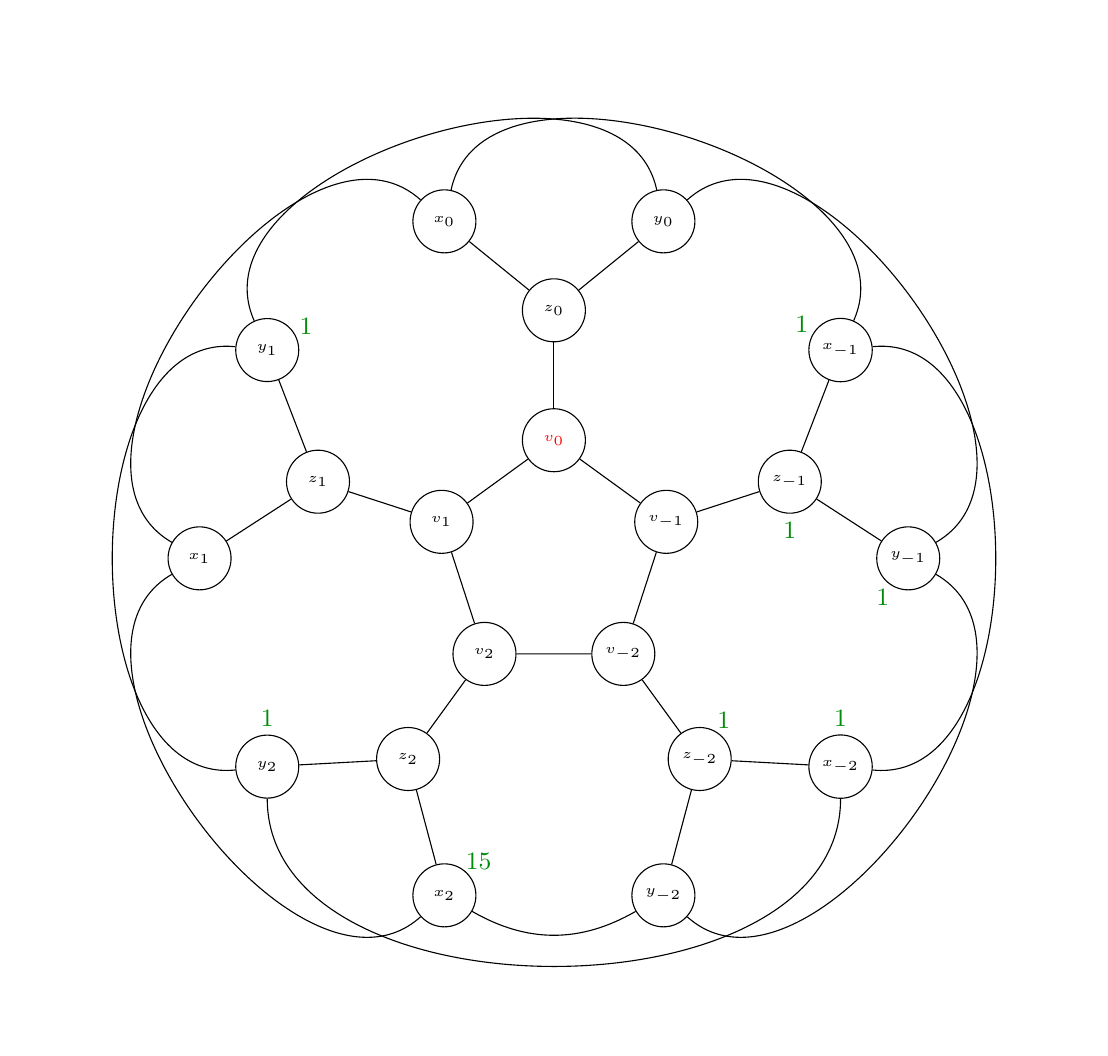
\begin{tikzpicture}[scale=0.75]
\tikzstyle{every node}=[draw,shape=circle,minimum size=.8cm,font=\tiny];
\def \Ang {360/5}
\def \ang {\Ang/4}
\def \radv {2cm}
\def \radz {4.2cm}
\def \radx {6cm}
% ----------
\path ({90 + (\Ang * 2)}:\radv) node (v2) {$v_2$};
\path ({90 + (\Ang * 1)}:\radv) node (v1) {$v_1$};
\path ({90 + (\Ang * 0)}:\radv) node (v0) {\color{red} $v_0$};
\path ({90 - (\Ang * 1)}:\radv) node (vm1) {$v_{-1}$};
\path ({90 - (\Ang * 2)}:\radv) node (vm2) {$v_{-2}$};
% ----------
\draw (v0) -- (vm1) -- (vm2) -- (v2) -- (v1) -- (v0);
% ----------
\path ({90 + (\Ang * 2)}:\radz) node (z2) {$z_2$};
\path ({90 + (\Ang * 1)}:\radz) node (z1) {$z_1$};
\path ({90 + (\Ang * 0)}:\radz) node (z0) {$z_0$};
\node[label={[label distance=-2mm]-90:{\color{gren}\small $1$}}] at ({90 - (\Ang * 1)}:\radz) (zm1) {$z_{-1}$};
\node[label={[label distance=-2mm]85:{\color{gren}\small $1$}}] at ({90 - (\Ang * 2)}:\radz) (zm2) {$z_{-2}$};
% ----------
\draw (v2) -- (z2);
\draw (v1) -- (z1);
\draw (v0) -- (z0);
\draw (vm1) -- (zm1);
\draw (vm2) -- (zm2);
% ----------
\node[label={[label distance=-2mm]45:{\color{gren}\small $15$}}] at ({90 + \ang + (\Ang * 2)}:\radx) (x2) {$x_2$};
\path ({90 + \ang + (\Ang * 1)}:\radx) node (x1) {$x_1$};
\path ({90 + \ang + (\Ang * 0)}:\radx) node (x0) {$x_0$};
\node[label={[label distance=-2mm]170:{\color{gren}\small $1$}}] at ({90 + \ang - (\Ang * 1)}:\radx) (xm1) {$x_{-1}$};
\node[label={[label distance=-2mm]90:{\color{gren}\small $1$}}] at ({90 + \ang - (\Ang * 2)}:\radx) (xm2) {$x_{-2}$};
% ----------
\node[label={[label distance=-2mm]90:{\color{gren}\small $1$}}] at ({90 - \ang + (\Ang * 2)}:\radx) (y2) {$y_2$};
\node[label={[label distance=-2mm]5:{\color{gren}\small $1$}}] at ({90 - \ang + (\Ang * 1)}:\radx) (y1) {$y_1$};
\path ({90 - \ang + (\Ang * 0)}:\radx) node (y0) {$y_0$};
\node[label={[label distance=-2mm]-100:{\color{gren}\small $1$}}] at ({90 - \ang - (\Ang * 1)}:\radx) (ym1) {$y_{-1}$};
\path ({90 - \ang - (\Ang * 2)}:\radx) node (ym2) {$y_{-2}$};
% ----------
\draw (x2) -- (z2) -- (y2);
\draw (x1) -- (z1) -- (y1);
\draw (x0) -- (z0) -- (y0);
\draw (xm1) -- (zm1) -- (ym1);
\draw (xm2) -- (zm2) -- (ym2);
% ----------
\draw (x2) to[out=-138,in=-150] (x1);
\draw (x1) to[out=150,in=138] (x0);
\draw (x0) to[out=78,in=66] (xm1);
\draw (xm1) to[out=6,in=-6] (xm2);
\draw (xm2) to[out=-90,in=-90] (y2);
% ----------
\draw (y2) to[out=-174,in=174] (y1);
\draw (y1) to[out=114,in=102] (y0);
\draw (y0) to[out=42,in=30] (ym1);
\draw (ym1) to[out=-30,in=-42] (ym2);
\draw (ym2) to[out=-150,in=-30] (x2);
% ----------
\end{tikzpicture}
\caption{The graph $J_{5}$ and its (green) $v_0$-unsolvable configuration $C$ of size $22$, which equals the configuration $C^*$ with an extra pebble on $z_{-1}$.}
\label{f:J5}
\end{figure}

For odd $m=2k+1$, we define the $m^{\rm th}$ {\it flower snark} $J_m$ as follows (see Figure~\ref{f:J5})~\cite{Campos}. 
For each $i\in\pm\{0,1,\ldots,k\}$ we have vertices $v_i$, $x_i$, and $y_i$ all adjacent to $z_i$.
Thus the number of vertices of the $m^{\rm th}$ flower snark is $n(J_m)=4m$.
The vertices $\{u_i\}$ form the natural cycle, with adjacencies given by consecutive indices modulo $m$.
The vertices $\{x_k\}$ (resp. $\{y_i\}$) form a path given by the natural cycle without the edge $x_kx_{-k}$ (resp. $y_ky_{-k}$).
Finally, we add the edges $x_ky_{-k}$ and $y_kx_{-k}$.
It is easy to see that $J_m$ has a rotational symmetry, with a necessary twist; that is, the automorphisms of $J_m$ yield three vertex orbits.
Thus the only targets necessary to contemplate are, without loss of generality, $v_0$, $z_0$, and $x_0$.

%=======================
%       RESULTS
%=======================
\subsection{Results}

It is known that the Petersen graph is Class 0 \cite{glenn1}.
It is %also 
the smallest snark and was the only one whose pebbling number is known (we now also know $\pi(J_3)$.)
%, below).
%
We use the Small Neighborhood Lemma below to prove that the Petersen graph is the only Class 0 snark with at least $23$ vertices or girth at least $5$.

\begin{thm}
\label{t:Petersen}
If a snark $G$ is \emph{Class 0} then either it is the Petersen graph, or $n(G)\le 22$ and ${\sf girth}(G)\le 4$.
\end{thm}

We also prove the following bounds on the pebbling numbers of snarks.

\begin{thm}
\label{t:Flower}
We have $\pi(J_3)=13$, $23\le \pi(J_5)\le 45$, $40\le \pi(J_7)\le 84$, and for all $k\ge 4$ with $m=2k+1$, we have $2^{k+2}+8\le \pi(J_m)\le (93\cdot 2^{k-1}+2)/5+2k-3$.
\end{thm}

This corrects a claim of \cite{pebblingflowersnark} that $\pi(J_{m})=4m+1$.


%%%%%%%%%%%%%%%%%%%%%%%%%%%%%%%%%%%%%%%%%%%%%%%
%       TECHNIQUES
%%%%%%%%%%%%%%%%%%%%%%%%%%%%%%%%%%%%%%%%%%%%%%%
\section{Techniques}

The following lemma (SNL) is used to provide a lower bound on $\pi(G)$.

\begin{lem}[Small Neighborhood Lemma \cite{cranston}]
Let $G$ be a graph and $u, v \in V(G)$. If $N_a[u] \cap N_b[v]=\emptyset$ and $\left|N_a[u] \cup N_b[v]\right|<2^{a+b+1}$, then $G$ is not Class 0.
\label{l:SNL}
\end{lem}

Given a graph $G$ that satisfies the hypothesis of Lemma \ref{l:SNL}, define the configuration $C^*=C^*_{u,v}$ by $C^*(v)=2^{a+b+1}-1$, $C^*(x)=0$ for all $x\in (N_x[u]\cup N_b[v])-\{v\}$, and $C^*(z)=1$ otherwise.
The authors of \cite{cranston} use the first hypothesis to prove that $C^*$ is $u$-unsolvable and the second hypothesis to show that $|C^*|\ge n(G)$.  In fact, we will use this configuration to get even larger lower bounds below.

One can see how SNL is, in some sense, a sharpening of the basic exponential lower bound.
One consequence we will use here is the following corollary.

\begin{cor}[\cite{cranston}]
\label{c:cranston}
If $G$ is an n-vertex Class 0 graph with diameter at least~3, then $e(G) \geq$ $\frac{5}{3} n-\frac{11}{3}$.
\end{cor}

Let $T$ be a subtree of a graph $G$ rooted at vertex $r$, with at least two vertices. 
For a vertex $v \in V(T)$ let $v^{+}$ denote the {\it parent} of $v$; i.e. the $T$-neighbor of $v$ that is one step closer to $r$ (we also say that $v$ is a {\it child} of $v^{+}$). 
We call $T$ an $r$-{\it strategy} when we associate with it a non-negative {\it weight function} $w$ with the property that $w(r)=0$ and $w\left(v^{+}\right) \ge 2 w(v)$ for every other vertex that is not a neighbor of $r$ (and $w(v)=0$ for vertices not in $T$ ). 
Let $\bT$ be the configuration with $\bT(r)=0, \bT(v)=1$ for all $v \in V(T)$, and $\bT(v)=0$ everywhere else. 
We now define the {\it weight} of any configuration $C$ (including $\bT$) by $w(C)=\sum_{v \in V} w(v) C(v)$.
The following lemma (WFL) is used to provide an upper bound on $\pi(G)$.


\begin{lem}[Weight Function Lemma \cite{HurlbertWFL}]
\label{l:WFL}
Let $T$ be an $r$-strategy of $G$ with associated weight function $w$. 
Suppose that $C$ is an $r$-unsolvable configuration of pebbles on $V(G)$. 
Then $w(C) \leq w(\bT)$.
\end{lem}


%%%%%%%%%%%%%%%%%%%%%%%%%%%%%%%%%%%%%%%%%%%%%%%
%       PETERSEN PROOF
%%%%%%%%%%%%%%%%%%%%%%%%%%%%%%%%%%%%%%%%%%%%%%%
\section{Proof of Theorem \ref{t:Petersen}}
\label{s:Petersen}
Note that every snark has $3n/2$ edges and diameter at least 3. 
Then, by Corollary \ref{c:cranston}, if $n(G)>22$ we get $3n/2 < (5n-11)/3$.
Therefore, every snark with $n(G)>22$ is not Class $0$.
The remaining non-Petersen snarks with fewer vertices and girth at least $5$ (the flower $J_5$, the Blanu\v{s}as, and the Loupekines) all have diameter $4$, so for any vertices $u$ and $v$ at distance 4 from each other we have $|N_2[u]|=10$ and $|N_1[v]|=4$.
Thus $\left|N_2[u] \cup N_1[v]\right|<2^{2+1+1} = 14<16$, and so none of these graphs are Class $0$ by SNL.
\hfill $\Box$


%%%%%%%%%%%%%%%%%%%%%%%%%%%%%%%%%%%%%%%%%%%%%%%
%       FLOWER PROOF
%%%%%%%%%%%%%%%%%%%%%%%%%%%%%%%%%%%%%%%%%%%%%%%
\section{Proof of Theorem \ref{t:Flower}}
\label{s:Flower}

First we prove the lower bounds.
For these we need only display a configuration, of size one less than the lower bound, that cannot reach some target.

For $J_3$, define the size $12$ configuration $C$ by $C(x_1)=7$, $C(u)=1$ for $u\in\{y_0,y_1,z_{-1},x_{-1},y_{-1}\}$, and $C(u)=0$ otherwise.
We claim that $C$ cannot reach $v_0$.
Indeed, $7$ pebbles cannot reach $v_0$ at distance $3$ without the assistance of other pebbles.
If we move a pebble from $x_1$ to its only nonempty neighbor $y_{-1}$ it can continue through other nonempty vertices until it reaches $z_0$, $z_1$, or $v_{-1}$, none of which can help the remaining $5$ pebbles on $x_1$ to reach $v_0$.
Otherwise, we do not move to $y_{-1}$, and the analysis is simpler.

For $J_5$, the $v_0$-unsolvable configuration $C^*_{v_0,x_k}$ that is provided by SNL has size 21.
Notice that we can add a pebble to $z_{-1}$ to obtain the configuration $C$ in Figure~\ref{f:J5}.
It is not difficult to argue that $C$ is also $v_0$-unsolvable, since any supposed solution would need to use the pebble at $z_{-1}$.

For $m\ge 7$ (i.e. $k\ge 3$), we will use $C^*=C^*_{v_0,x_k}$ only.
One can verify that, for any vertex $u$ of $J_m$ and integer $2\le i\le k$, we have $|N_i[u]|=2(4i-5)+4=8i-6$.
From this we can compute $|C^*|=(2^{a+b+1}-1) + (n - |N_a[v_0]| - |N_b[x_k]|)$.
In the case that $k$ is even we use $a=k/2$ and $b=a+1$, while if $k$ is odd we use $a=b=(k+1)/2$.
In either case we obtain $|C^*|=2^{k+2}+8$.

Now we prove the upper bounds, using WFL.
For $J_3$, we define three $v_0$-strategies $\bT_0$, $\bT_1$, and $\bT_{-1}$ by 
\vspace{-0.04in}
\begin{quote}
    $\bullet$ 
    $\bT_0(z_0,x_0,y_0,x_1,y_1,x_{-1},y_{-1},z_1,z_{-1}) = (8,4,4,2,2,2,2,1,1)$, \\
    $\bullet$
    $\bT_1(v_1,z_1,x_1,y_1,x_0,x_{-1},y_{-1}) = (8,4,2,2,1,1,1)$ and\\ 
    $\bullet$
    $\bT_{-1}(v_{-1},z_{-1},x_{-1},y_{-1},y_0,x_1,y_1) = (8,4,2,2,1,1,1)$,
\end{quote}
giving rise to the inequality $|C| \le \frac{1}{5}(\bT_0+\bT_1+\bT_{-1}) \le 64/5$ whenever $C$ is $v_0$-unsolvable.
Hence $\pi(J_3,v_0)\le 13$.
Similar strategies can be found for targets $z_0$ and $x_0$ as well, and so $\pi(J_3)\le 13$.

For $m\in\{5,7\}$, we define $v_0$-strategies similarly.
For $m\ge 9$ (i.e. $k\ge 4$), we instead define three $z_0$-strategies (see Figure \ref{f:J11}) by
\begin{itemize}
    \item 
    $\bT_0(v_0,v_1,v_{-1},v_2,v_{-2},\ldots, v_k,v_{-k},z_k,z_{-k},x_k,y_k,x_{-k},y_{-k})$\\
    $= (2^{k+2},2^{k+1},2^{k+1},2^k,2^k,\ldots, 2,2,1,1,1,1)$ and\\
    $\bT_0(z_1,z_{-1},\ldots,z_{k-2},z_{2-k},z_{k-1},z_{1-k})
    = (5,5,\ldots,5,5,4,4)$;
    \item
    $\bT_1(x_0,x_1,x_{-1},\ldots,x_k,x_{-k},z_k,v_k)\\
    = (2^{k+2},2^{k+1},2^{k+1},\ldots,4,4,2,1)$ and\\
    $\bT_1(z_{2-k},z_{1-k}) = (1,1)$; and
    \item
    $\bT_{-1}(y_0,y_1,y_{-1},\ldots,y_k,y_{-k},z_{-k},v_{-k})\\
    = (2^{k+2},2^{k+1},2^{k+1},\ldots,4,4,2,1)$ and\\
    $\bT_{-1}(z_{k-2},z_{k-1}) = (1,1)$.
\end{itemize}

\begin{figure}%[bht]
\centering
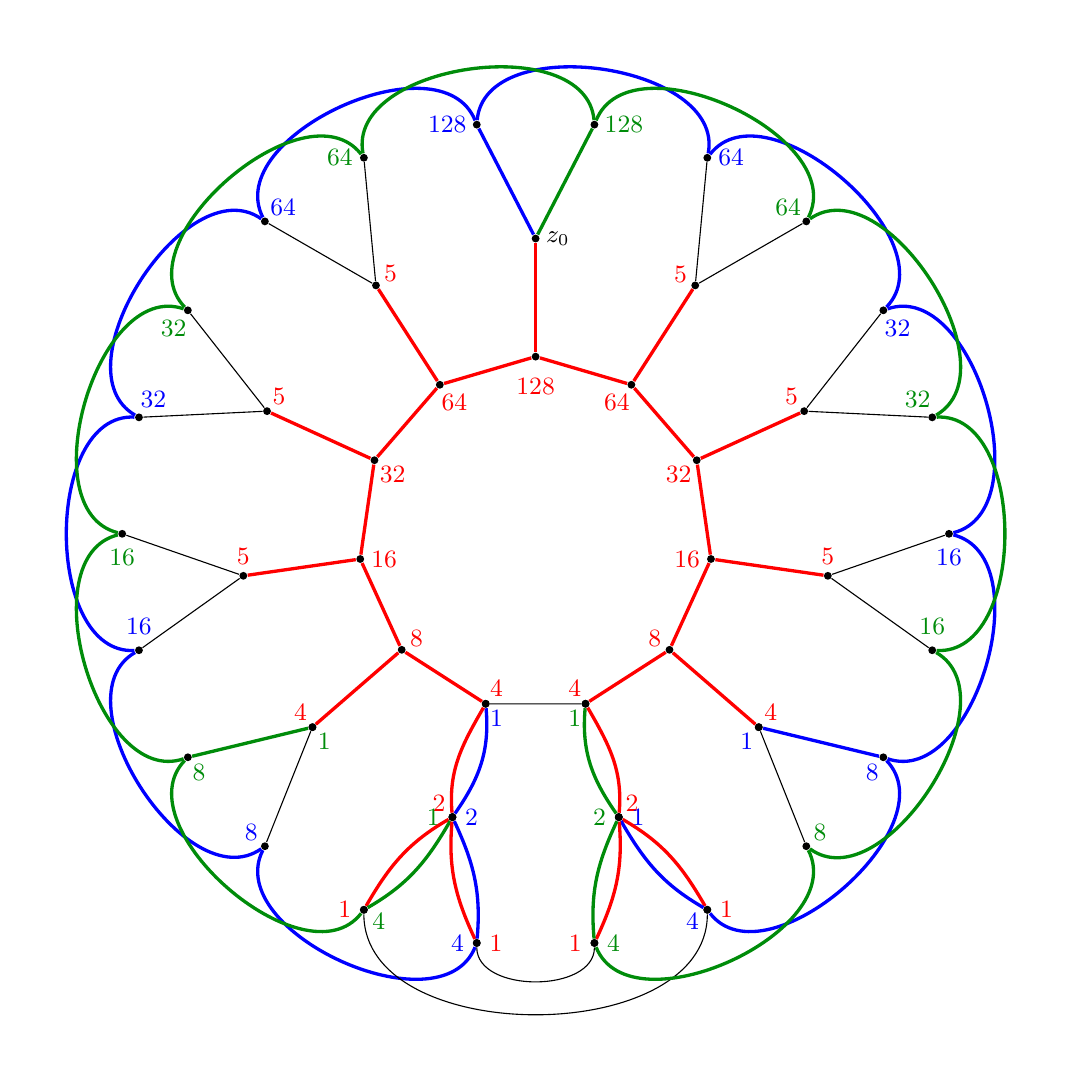
\begin{tikzpicture}[scale=1.5]
\tikzstyle{every node}=[circle,fill=black,inner sep=1pt];
\def \Ang {360/11}
\def \ang {\Ang/4}
\def \radv {1.5cm}
\def \radz {2.5cm}
\def \radx {3.5cm}
% ----------
\node[label={85:{\color{red}\small $4$}}] at ({90 + (\Ang * 5)}:\radv) (v5) {};
\node[label={-85:{\color{blue}\small $1$}}] at ({90 + (\Ang * 5)}:\radv) (v5b) {};
\node[label={10:{\color{red}\small $8$}}] at ({90 + (\Ang * 4)}:\radv) (v4) {};
\node[label={0:{\color{red}\small $16$}}] at ({90 + (\Ang * 3)}:\radv) (v3) {};
\node[label={-10:{\color{red}\small $32$}}] at ({90 + (\Ang * 2)}:\radv) (v2) {};
\node[label={280:{\color{red}\small $64$}}] at ({90 + (\Ang * 1)}:\radv) (v1) {};
\node[label={270:{\color{red}\small $128$}}] at ({90 + (\Ang * 0)}:\radv) (v0) {};
\node[label={260:{\color{red}\small $64$}}] at ({90 - (\Ang * 1)}:\radv) (vm1) {};
\node[label={190:{\color{red}\small $32$}}] at ({90 - (\Ang * 2)}:\radv) (vm2) {};
\node[label={180:{\color{red}\small $16$}}] at ({90 - (\Ang * 3)}:\radv) (vm3) {};
\node[label={170:{\color{red}\small $8$}}] at ({90 - (\Ang * 4)}:\radv) (vm4) {};
\node[label={95:{\color{red}\small $4$}}] at ({90 - (\Ang * 5)}:\radv) (vm5) {};
\node[label={-95:{\color{gren}\small $1$}}] at ({90 - (\Ang * 5)}:\radv) (vm5g) {};
% ----------
\draw[very thick,red] (v0) -- (vm1) -- (vm2) -- (vm3) -- (vm4) -- (vm5);
\draw[very thick,red] (v5) -- (v4) -- (v3) -- (v2) -- (v1) -- (v0);
\draw (vm5) -- (v5);
% ----------
\node[label={0:{\color{blue}\small $2$}}] at ({90 + (\Ang * 5)}:\radz) (z5) {};
\node[label={130:{\color{red}\small $2$}}] at ({90 + (\Ang * 5)}:\radz) (z5r) {};
\node[label={180:{\color{gren}\small $1$}}] at ({90 + (\Ang * 5)}:\radz) (z5g) {};
\node[label={110:{\color{red}\small $4$}}] at ({90 + (\Ang * 4)}:\radz) (z4) {};
\node[label={290:{\color{gren}\small $1$}}] at ({90 + (\Ang * 4)}:\radz) (z4g) {};
\node[label={90:{\color{red}\small $5$}}] at ({90 + (\Ang * 3)}:\radz) (z3) {};
\node[label={70:{\color{red}\small $5$}}] at ({90 + (\Ang * 2)}:\radz) (z2) {};
\node[label={20:{\color{red}\small $5$}}] at ({90 + (\Ang * 1)}:\radz) (z1) {};
\node[label={0:{\small $z_0$}}] at ({90 - (\Ang * 0)}:\radz) (z0) {};
\node[label={170:{\color{red}\small $5$}}] at ({90 - (\Ang * 1)}:\radz) (zm1) {};
\node[label={120:{\color{red}\small $5$}}] at ({90 - (\Ang * 2)}:\radz) (zm2) {};
\node[label={90:{\color{red}\small $5$}}] at ({90 - (\Ang * 3)}:\radz) (zm3) {};
\node[label={70:{\color{red}\small $4$}}] at ({90 - (\Ang * 4)}:\radz) (zm4) {};
\node[label={250:{\color{blue}\small $1$}}] at ({90 - (\Ang * 4)}:\radz) (zm4b) {};
\node[label={180:{\color{gren}\small $2$}}] at ({90 - (\Ang * 5)}:\radz) (zm5) {};
\node[label={50:{\color{red}\small $2$}}] at ({90 - (\Ang * 5)}:\radz) (zm5g) {};
\node[label={0:{\color{blue}\small $1$}}] at ({90 - (\Ang * 5)}:\radz) (zm5b) {};
% ----------
\draw[very thick,blue] (v5) to[out=275,in=55] (z5);
\draw[very thick,red] (v5) to[out=240,in=95] (z5);
\draw[very thick,red] (v4) -- (z4);
\draw[very thick,red] (v3) -- (z3);
\draw[very thick,red] (v2) -- (z2);
\draw[very thick,red] (v1) -- (z1);
\draw[very thick,red] (v0) -- (z0);
\draw[very thick,red] (vm1) -- (zm1);
\draw[very thick,red] (vm2) -- (zm2);
\draw[very thick,red] (vm3) -- (zm3);
\draw[very thick,red] (vm4) -- (zm4);
\draw[very thick,gren] (vm5) to[out=265,in=125] (zm5);
\draw[very thick,red] (vm5) to[out=300,in=85] (zm5);
% ----------
\node[label={180:{\color{blue}\small $4$}}] at ({90 + \ang + (\Ang * 5)}:\radx) (x5) {};
\node[label={0:{\color{red}\small $1$}}] at ({90 + \ang + (\Ang * 5)}:\radx) (x5r) {};
\node[label={135:{\color{blue}\small $8$}}] at ({90 + \ang + (\Ang * 4)}:\radx) (x4) {};
\node[label={90:{\color{blue}\small $16$}}] at ({90 + \ang + (\Ang * 3)}:\radx) (x3) {};
\node[label={80:{\color{blue}\small $32$}}] at ({90 + \ang + (\Ang * 2)}:\radx) (x2) {};
\node[label={5:{\color{blue}\small $64$}}] at ({90 + \ang + (\Ang * 1)}:\radx) (x1) {};
\node[label={180:{\color{blue}\small $128$}}] at ({90 + \ang + (\Ang * 0)}:\radx) (x0) {};
\node[label={0:{\color{blue}\small $64$}}] at ({90 + \ang - (\Ang * 1)}:\radx) (xm1) {};
\node[label={-85:{\color{blue}\small $32$}}] at ({90 + \ang - (\Ang * 2)}:\radx) (xm2) {};
\node[label={-90:{\color{blue}\small $16$}}] at ({90 + \ang - (\Ang * 3)}:\radx) (xm3) {};
\node[label={-100:{\color{blue}\small $8$}}] at ({90 + \ang - (\Ang * 4)}:\radx) (xm4) {};
\node[label={190:{\color{blue}\small $4$}}] at ({90 + \ang - (\Ang * 5)}:\radx) (xm5) {};
\node[label={0:{\color{red}\small $1$}}] at ({90 + \ang - (\Ang * 5)}:\radx) (xm5r) {};
% ----------
\node[label={-10:{\color{gren}\small $4$}}] at ({90 - \ang + (\Ang * 5)}:\radx) (y5) {};
\node[label={180:{\color{red}\small $1$}}] at ({90 - \ang + (\Ang * 5)}:\radx) (y5r) {};
\node[label={-80:{\color{gren}\small $8$}}] at ({90 - \ang + (\Ang * 4)}:\radx) (y4) {};
\node[label={-90:{\color{gren}\small $16$}}] at ({90 - \ang + (\Ang * 3)}:\radx) (y3) {};
\node[label={265:{\color{gren}\small $32$}}] at ({90 - \ang + (\Ang * 2)}:\radx) (y2) {};
\node[label={180:{\color{gren}\small $64$}}] at ({90 - \ang + (\Ang * 1)}:\radx) (y1) {};
\node[label={0:{\color{gren}\small $128$}}] at ({90 - \ang - (\Ang * 0)}:\radx) (y0) {};
\node[label={175:{\color{gren}\small $64$}}] at ({90 - \ang - (\Ang * 1)}:\radx) (ym1) {};
\node[label={100:{\color{gren}\small $32$}}] at ({90 - \ang - (\Ang * 2)}:\radx) (ym2) {};
\node[label={90:{\color{gren}\small $16$}}] at ({90 - \ang - (\Ang * 3)}:\radx) (ym3) {};
\node[label={45:{\color{gren}\small $8$}}] at ({90 - \ang - (\Ang * 4)}:\radx) (ym4) {};
\node[label={0:{\color{gren}\small $4$}}] at ({90 - \ang - (\Ang * 5)}:\radx) (ym5) {};
\node[label={180:{\color{red}\small $1$}}] at ({90 - \ang - (\Ang * 5)}:\radx) (ym5r) {};
% ----------
\draw[very thick,red] (y5) to[out=60,in=210] (z5);
\draw[very thick,gren] (y5) to[out=30,in=240] (z5);
\draw[very thick,red] (x5) to[out=115,in=265] (z5);
\draw[very thick,blue] (x5) to[out=85,in=295] (z5);
\draw (x4) -- (z4);
\draw[very thick,gren] (z4) -- (y4);
\draw (x3) -- (z3) -- (y3);
\draw (x2) -- (z2) -- (y2);
\draw (x1) -- (z1) -- (y1);
\draw[very thick,blue] (x0) -- (z0);
\draw[very thick,gren] (z0) -- (y0);
\draw (xm1) -- (zm1) -- (ym1);
\draw (xm2) -- (zm2) -- (ym2);
\draw (xm3) -- (zm3) -- (ym3);
\draw[very thick,blue] (xm4) -- (zm4);
\draw (zm4) -- (ym4);
\draw[very thick,red] (zm5) to[out=330,in=120] (xm5);
\draw[very thick,blue] (zm5) to[out=300,in=150] (xm5);
\draw[very thick,red] (zm5) to[out=275,in=65] (ym5);
\draw[very thick,gren] (zm5) to[out=245,in=95] (ym5);
% ----------
\draw[very thick,blue] (x5) to[out=248,in=243] (x4);
\draw[very thick,blue] (x4) to[out=215,in=210] (x3);
\draw[very thick,blue] (x3) to[out=183,in=177] (x2);
\draw[very thick,blue] (x2) to[out=150,in=145] (x1);
\draw[very thick,blue] (x1) to[out=117,in=112] (x0);
\draw[very thick,blue] (x0) to[out=85,in=79] (xm1);
\draw[very thick,blue] (xm1) to[out=52,in=46] (xm2);
\draw[very thick,blue] (xm2) to[out=19,in=14] (xm3);
\draw[very thick,blue] (xm3) to[out=-14,in=-19] (xm4);
\draw[very thick,blue] (xm4) to[out=-46,in=-52] (xm5);
\draw (xm5) to[out=-90,in=-90] (y5);
% ----------
\draw[very thick,gren] (y5) to[out=232,in=226] (y4);
\draw[very thick,gren] (y4) to[out=199,in=194] (y3);
\draw[very thick,gren] (y3) to[out=166,in=161] (y2);
\draw[very thick,gren] (y2) to[out=134,in=128] (y1);
\draw[very thick,gren] (y1) to[out=101,in=95] (y0);
\draw[very thick,gren] (y0) to[out=68,in=63] (ym1);
\draw[very thick,gren] (ym1) to[out=35,in=30] (ym2);
\draw[very thick,gren] (ym2) to[out=3,in=-3] (ym3);
\draw[very thick,gren] (ym3) to[out=-30,in=-36] (ym4);
\draw[very thick,gren] (ym4) to[out=-63,in=-68] (ym5);
\draw (ym5) to[out=-90,in=-90] (x5);
% ----------
\end{tikzpicture}
\caption{The graph $J_{11}$ and its three $z_0$-strategies $\bT_0$ (in red), $\bT_1$ (in blue), and $\bT_{-1}$ (in green).}
\label{f:J11}
\end{figure}

The sum $\bT_0+\bT_1+\bT_{-1}$ has $3$ vertices with coefficient $2^{k+2}$, $6$ with $2^i$ (for each $3\le i\le k+1$), and $2k+6$ with coefficient $5$, giving rise to the inequality 
\begin{align*}
    5|C|
    &\le \bT_0+\bT_1+\bT_{-1}\\
    &= 6(2^3 + \cdots + 2^{k+2}) - 3(2^{k-1}) + 5(2k+6)\\
    &= 48(2^k-1) - 3(2^{k-1}) + 10k + 30\\
    &= 93(2^{k-1}) + 10k - 18,
\end{align*}
whenever $C$ is $v_0$-unsolvable.
Hence $|C|\le (93\cdot 2^{k-1} + 2)/5 + 2k - 4$, and so $\pi(J_m,z_0)\le (93\cdot 2^{k-1} + 2)/5 + 2k - 3$.
Similar strategies can also be found for targets $v_0$ and $x_0$, and so $\pi(J_m)\le (93\cdot 2^{k-1} + 2)/5 + 2k - 3$.
\hfill $\Box$


%%%%%%%%%%%%%%%%%%%%%%%%%%%%%%%%%%%%%%%%%%%%%%%
%       REMARKS
%%%%%%%%%%%%%%%%%%%%%%%%%%%%%%%%%%%%%%%%%%%%%%%
\section{Final remarks}

Table \ref{snarktable} shows the current knowledge of the pebbling numbers of several well known snarks, using the basic bounds mentioned in the introduction, as well as Theorems \ref{t:Petersen} and \ref{t:Flower}.
We also note that the Watkins lower bound comes from a more complicated argument that will be included in a follow-up article, correcting a claim of \cite{pebblingwatkinssnark} that $\pi(W_{50})=166$.

\begin{table}%[h!]
\resizebox{\textwidth}{!}{
\begin{tabular}{|l|c|c|c|}
\hline
&&&\\
Snark & $n(G)$ & $D(G)$ & $\pi(G)$ \\
&&&\\
\hline
&&&\\
Petersen & 10 & 3 & 10 \\ 
&&&\\
\hline
&&&\\
Flower $J_3$ & 12 & 3 & 13 \\
&&&\\
\hline
&&&\\
Flower $J_5$ & 20 & 4 & $23\le \pi(J_5)\le 45$ \\
&&&\\
\hline
&&&\\
Flower $J_7$ & 28 & 5 & $40\le \pi(J_5)\le 84$ \\
&&&\\
\hline
&&&\\
Flower $J_m$ ($m\ge 9$) & $4m$ & $(m-1)/2$ & $2^{k+2}+8\le \pi(J_m)\le (93\cdot 2^{k-1}+2)/5+2k-3$ \\
&&&\\
\hline
&&&\\
Blanu\v{s}a (1 and 2) & 18 & 4 & $ 19 \le \pi(G) \leq 211$ \\
&&&\\
\hline
&&&\\
Loupekine (1 and 2) & 22 & 4 & $23 \le \pi(G) \leq 271$ \\
&&&\\
\hline
&&&\\
Double-Star & 30 & 4 & $31 \le \pi(G) \leq 391$ \\
&&&\\
\hline
&&&\\
Szekeres & 50 & 7 & $128 \le \pi(G) \leq 5462$ \\
&&&\\
\hline
&&&\\
Watkins & 50 & 7 & $169 \le \pi(G) \leq 5462$ \\
&&&\\
\hline
\end{tabular}}
\caption{Bounds on the pebbling numbers of several well known snarks.}
\label{snarktable}
\end{table}


%%%%%%%%%%%%%%%%%%%%%%%%%%%%%%%%%%%%%%%%%%%%%%%
%       ACKNOWLEDGEMENTS
%%%%%%%%%%%%%%%%%%%%%%%%%%%%%%%%%%%%%%%%%%%%%%%
\section*{Acknowledgements}

This research was partially supported by CAPES  Finance Code 001, FAPERJ (grant no. E-26/202.793/2017, E-26/010.002239/201), and CNPq (grant
no. 407635/2018-1, 305356/2021-6).

\newpage


%%%%%%%%%%%%%%%%%%%%%%%%%%%%%%%%%%%%%%%%%%%%%%%
%           BIBLIO
%%%%%%%%%%%%%%%%%%%%%%%%%%%%%%%%%%%%%%%%%%%%%%%

\bibliography{database-doses}
\bibliographystyle{acm}
\nocite{caroll}
\nocite{gard}

\end{document}

